\documentclass[11pt]{article}
\usepackage[letterpaper,margin=1.45cm]{geometry}
\usepackage{tikz}
\usepackage{amsmath,amssymb}
\usepackage[T1]{fontenc}
\usepackage{lmodern}
\usepackage{enumitem}
\usepackage{array}
\usepackage{fancyhdr}
\usepackage{xcolor}
\setlength{\parindent}{0pt}
\pagestyle{fancy}
\fancyhf{}
\lhead{Geometry 8 - Circle Fundamentals}
\rhead{Notebook Guide}
\cfoot{\thepage}
\renewcommand{\headrulewidth}{0.4pt}
\definecolor{softgray}{gray}{0.93}
\newcommand{\Term}[1]{\vspace{0.1cm}{\Large\bfseries #1}\par\vspace{0.2cm}\hrule\vspace{0.45cm}}
\newcommand{\CopyBox}[1]{\begin{center}\fcolorbox{black}{white}{\begin{minipage}{0.90\linewidth}\textbf{COPY TO NOTEBOOK}\par\vspace{0.15cm}#1\end{minipage}}\end{center}}
\newcommand{\BlankLines}{\vspace{0.25cm}\foreach \x in {1,...,4}{\noindent\rule{\linewidth}{0.25pt}\vspace{0.47cm}}}
\begin{document}

\begin{center}
{\LARGE\bfseries CIRCLE FUNDAMENTALS}\par\vspace{0.35cm}
{\Large Center, radius, diameter, chords and arcs}\par\vspace{0.45cm}
{\large Geometry 8 - Notebook-copy edition}\par\vspace{0.7cm}
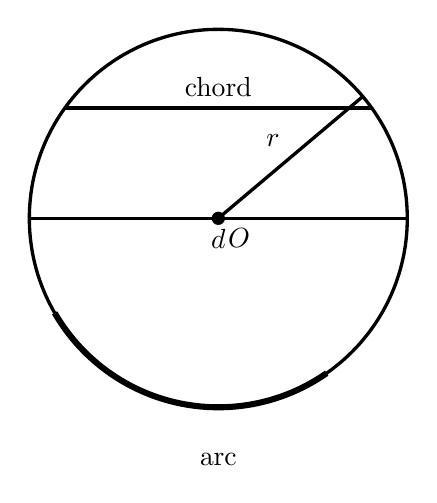
\begin{tikzpicture}[scale=1.2]
\draw[line width=1.2pt] (0,0) circle (2);
\fill (0,0) circle (2pt) node[below right] {$O$};
\draw[line width=1.2pt] (0,0)--(1.53,1.29) node[midway,above left] {$r$};
\draw[line width=1pt] (-2,0)--(2,0) node[midway,below] {$d$};
\draw[line width=1.4pt] (-1.62,1.17)--(1.62,1.17) node[midway,above] {chord};
\draw[line width=2.2pt] (210:2) arc[start angle=210,end angle=305,radius=2];
\node at (0,-2.55) {arc};
\end{tikzpicture}
\end{center}
\vfill
\textbf{Goal:} Identify each element by its shape and by the points it connects.\par
\textbf{Spanish glossary:} center = centro, radius = radio, diameter = di\'ametro, chord = cuerda, arc = arco.
\newpage

\Term{1. CENTER (O)}
\begin{minipage}[t]{0.47\linewidth}
\begin{center}
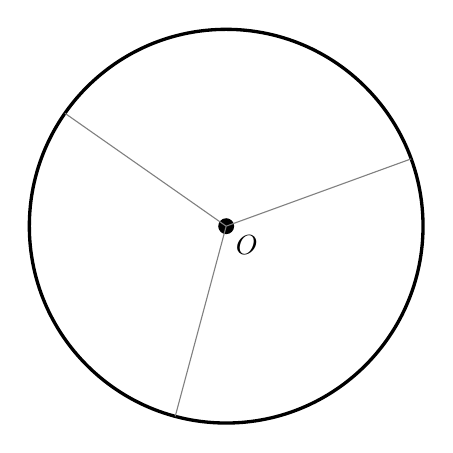
\begin{tikzpicture}[scale=1.25]
\draw[line width=1.2pt] (0,0) circle (2);
\fill (0,0) circle (2.3pt) node[below right] {$O$};
\draw[gray] (0,0)--(20:2);
\draw[gray] (0,0)--(145:2);
\draw[gray] (0,0)--(255:2);
\end{tikzpicture}
\end{center}
\end{minipage}\hfill
\begin{minipage}[t]{0.49\linewidth}
\CopyBox{The center is a fixed point inside the circle.\\[4pt]
Every point on the circumference is the same distance from $O$.}
\end{minipage}
\vspace{0.5cm}
\textbf{Key idea:} The center organizes the radius, diameter, chords and angle relationships of the circle.
\BlankLines
\newpage

\Term{2. RADIUS (r)}
\begin{minipage}[t]{0.47\linewidth}
\begin{center}
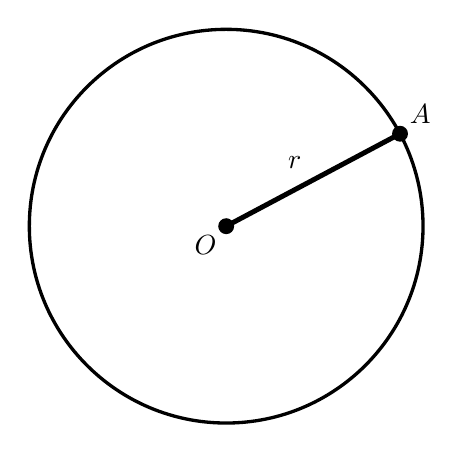
\begin{tikzpicture}[scale=1.25]
\draw[line width=1.2pt] (0,0) circle (2);
\fill (0,0) circle (2.3pt) node[below left] {$O$};
\coordinate (A) at (28:2);
\fill (A) circle (2.3pt) node[above right] {$A$};
\draw[line width=1.8pt] (0,0)--(A) node[midway,above left] {$r$};
\end{tikzpicture}
\end{center}
\end{minipage}\hfill
\begin{minipage}[t]{0.49\linewidth}
\CopyBox{A radius is a segment from the center to the circumference.\\[4pt]
All radii of the same circle have equal length.\\[6pt]
\[OA=r\]}
\end{minipage}
\vspace{0.5cm}
\textbf{How to recognize it:} one endpoint is the center; the other endpoint is on the circumference.
\BlankLines
\newpage

\Term{3. DIAMETER (d)}
\begin{minipage}[t]{0.47\linewidth}
\begin{center}
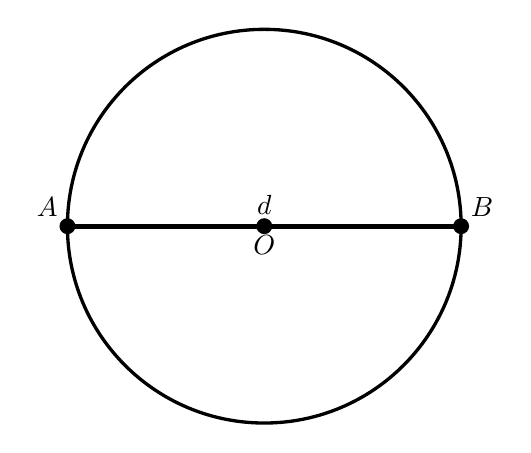
\begin{tikzpicture}[scale=1.25]
\draw[line width=1.2pt] (0,0) circle (2);
\fill (-2,0) circle (2.3pt) node[above left] {$A$};
\fill (0,0) circle (2.3pt) node[below] {$O$};
\fill (2,0) circle (2.3pt) node[above right] {$B$};
\draw[line width=1.8pt] (-2,0)--(2,0) node[midway,above] {$d$};
\end{tikzpicture}
\end{center}
\end{minipage}\hfill
\begin{minipage}[t]{0.49\linewidth}
\CopyBox{A diameter joins two points on the circumference.\\[4pt]
It passes through the center of the circle.\\[4pt]
One diameter contains two radii.\\[6pt]
\[d=2r \qquad r=\frac{d}{2}\]}
\end{minipage}
\vspace{0.4cm}
\textbf{Key idea:} A diameter is a special chord and the longest chord in a circle.
\BlankLines
\newpage

\Term{4. CHORD}
\begin{minipage}[t]{0.47\linewidth}
\begin{center}
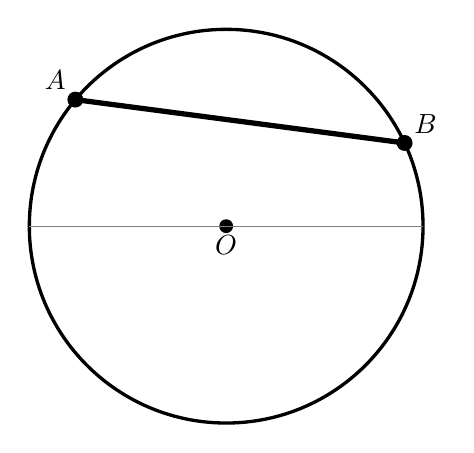
\begin{tikzpicture}[scale=1.25]
\draw[line width=1.2pt] (0,0) circle (2);
\fill (0,0) circle (2pt) node[below] {$O$};
\coordinate (A) at (140:2);
\coordinate (B) at (25:2);
\fill (A) circle (2.3pt) node[above left] {$A$};
\fill (B) circle (2.3pt) node[above right] {$B$};
\draw[gray] (-2,0)--(2,0);
\draw[line width=1.9pt] (A)--(B);
\end{tikzpicture}
\end{center}
\end{minipage}\hfill
\begin{minipage}[t]{0.49\linewidth}
\CopyBox{A chord is a segment joining two points on the circumference.\\[4pt]
A chord may or may not pass through the center.\\[4pt]
Every diameter is a chord, but not every chord is a diameter.}
\end{minipage}
\vspace{0.4cm}
\textbf{How to distinguish it from a diameter:} check whether the segment passes through $O$.
\BlankLines
\newpage

\Term{5. ARC}
\begin{minipage}[t]{0.47\linewidth}
\begin{center}
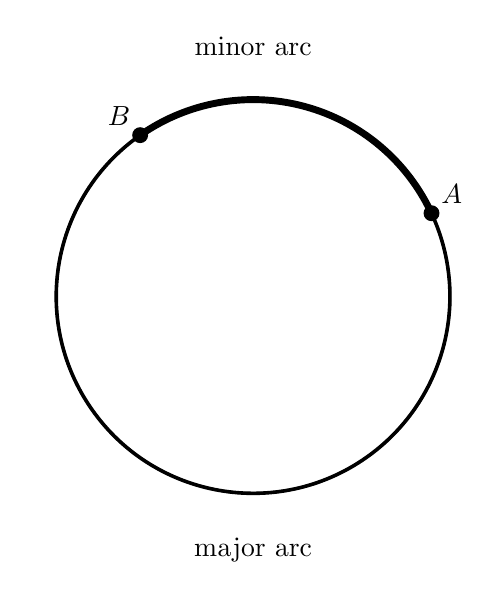
\begin{tikzpicture}[scale=1.25]
\draw[gray,line width=1pt] (0,0) circle (2);
\coordinate (A) at (25:2);
\coordinate (B) at (125:2);
\fill (A) circle (2.3pt) node[above right] {$A$};
\fill (B) circle (2.3pt) node[above left] {$B$};
\draw[line width=2.5pt] (25:2) arc[start angle=25,end angle=125,radius=2];
\draw[line width=1.3pt] (125:2) arc[start angle=125,end angle=385,radius=2];
\node[above] at (0,2.35) {minor arc};
\node[below] at (0,-2.35) {major arc};
\end{tikzpicture}
\end{center}
\end{minipage}\hfill
\begin{minipage}[t]{0.49\linewidth}
\CopyBox{An arc is part of the circumference between two points.\\[4pt]
A minor arc measures less than $180^\circ$.\\[4pt]
A major arc measures more than $180^\circ$.}
\end{minipage}
\vspace{0.4cm}
\textbf{Key idea:} A chord is straight; an arc is curved.
\BlankLines
\newpage

\Term{6. PUT THE FIVE ELEMENTS TOGETHER}
\begin{center}
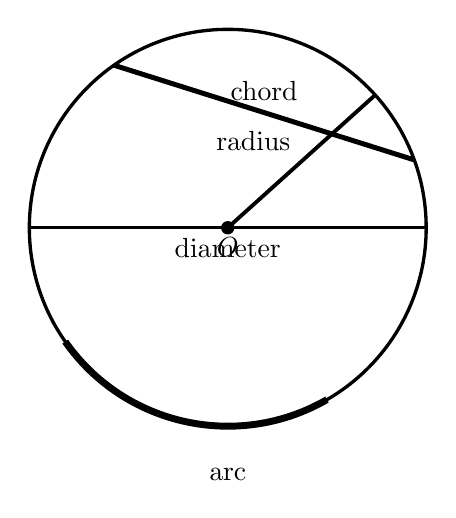
\begin{tikzpicture}[scale=1.05]
\draw[line width=1.2pt] (0,0) circle (2.4);
\fill (0,0) circle (2.3pt) node[below] {$O$};
\draw[line width=1.4pt] (0,0)--(42:2.4) node[midway,above left] {radius};
\draw[line width=1.0pt] (-2.4,0)--(2.4,0) node[midway,below] {diameter};
\draw[line width=1.8pt] (125:2.4)--(20:2.4) node[midway,above] {chord};
\draw[line width=2.5pt] (215:2.4) arc[start angle=215,end angle=300,radius=2.4];
\node[below] at (0,-2.8) {arc};
\end{tikzpicture}
\end{center}
\vspace{0.35cm}
\renewcommand{\arraystretch}{1.45}
\begin{center}
\begin{tabular}{|>{\bfseries}p{3.4cm}|p{10.2cm}|}\hline
CENTER & fixed point $O$ inside the circle \\ \hline
RADIUS & center to circumference \\ \hline
DIAMETER & two circumference points and passes through center \\ \hline
CHORD & two circumference points; may miss center \\ \hline
ARC & curved part of the circumference \\ \hline
\end{tabular}
\end{center}
\newpage

\Term{7. NOTEBOOK CHECK}
Write the correct element beside each clue.
\begin{enumerate}[leftmargin=1.1cm,itemsep=0.55cm]
\item Starts at $O$ and ends on the circumference. \hfill \rule{5cm}{0.3pt}
\item Joins two points and passes through $O$. \hfill \rule{5cm}{0.3pt}
\item Joins two points but may miss $O$. \hfill \rule{5cm}{0.3pt}
\item Curved part of the circumference. \hfill \rule{5cm}{0.3pt}
\item Fixed point equally distant from the circumference. \hfill \rule{5cm}{0.3pt}
\end{enumerate}
\vspace{0.8cm}
\textbf{Final memory route:}
\[
\boxed{\text{CENTER}}\;\longrightarrow\;\boxed{\text{RADIUS}}\;\longrightarrow\;\boxed{\text{DIAMETER}}\;\longrightarrow\;\boxed{\text{CHORD}}\;\longrightarrow\;\boxed{\text{ARC}}
\]
\vfill
\textit{Study rule: identify the endpoints and check whether the object is straight or curved.}

\end{document}
